\hypertarget{paper-1}{%
\chapter{Digital Trace Data as Indicators of the Social World: Validating Google Trends for use in Scientific Research}\label{paper-1}}

\section{Abstract}

Computational social science and disciplines such as sociology and political
science are often quick to adopt new sources of digital trace data for use in
academic research. In this article, I examine the criterion validity of Google
Search Trends as potential indicators of three different cases, namely
attitudes, disease prevalence and political preferences using five different
validated data sources. I use Pearson and Repeated Measures Correlations between
the Google Trends and the validated indicators as well as multiple linear
regression (for cross-sectional datasets) and fixed effect hierarchical linear
models (for longitudinal datasets) as additional tests of the data. I find no
correlation among any of the Google Trends tested and their validated
indicators. While some Google Trends tested were significantly associated with
the outcome in the regression models, effects tended to be small and the total
model interpretability remained low, even when controlling for demographic
variables. This article shows that there is no criterion validity of Google
Trends for these uses and social scientists are not able to use Google Trends as
a stand-in for high quality survey data.

\textbf{Keywords}: Google Trends, Social Science Methodology, Digital Trace Data, Information-Seeking Behavior, Information and communications technology, Validity

\section{Introduction}

New sources of digital trace data have led to vast possibilities for social
science research because they are bigger, cheaper, and already available
\citep{kingEnsuringDataRichFuture2011,lazerComputationalSocialScience2009,salganikBitBitSocial2017}.
Digital trace data are the expansive volumes of information that are now
available with the introduction and widespread adoption of the internet and
include sources such as social media sites, search data, blogs, administrative
data on websites, the internet archives, etc. In short, digital trace data are
the crumbs that are left as a person peruses and interacts in digital spaces.
Scholars have noted that these data provide many new research avenues for social
scientists because they are always on, non-reactive to a researcher's
observation, and very often capture social interactions and relationships, but
warn they can be inaccessible, non-representative, and be prone to drifting due
to algorithmic confounding\citep{salganikBitBitSocial2017}. Before
overenthusiastically embracing these sources and integrating them into our big
data toolkits, social scientists must clearly establish parameters under which
these data sources are appropriate, and for which questions they are useful
\citep{bailCulturalEnvironmentMeasuring2014, lazerParableGoogleFlu2014}. As
prior research outlined, the ``quantity of data does not mean that one can ignore
foundational issues of measurement and construct validity and reliability and
dependencies among data'' \citep[p. 1203]{lazerParableGoogleFlu2014}.

With the expansion of big data, some computational social science research has
developed extremely innovative methods that have led to groundbreaking results
using reliable sources of big data. As an
example,\citet{blumenstockPredictingPovertyWealth2015} use county-level
cell-phone records to construct the distribution of poverty and wealth in
Rwanda, a country where national surveys and censuses are rare and costly.
In this paper,  \citet{blumenstockPredictingPovertyWealth2015} put in an effort to 
investigate the criterion validity of their measure; that is, they investigate 
how well an \textit{operationalization} of a specific construct is able to 
predict a \textit{theoretical representation} of the construct — the criterion. 
Investigating the criterion validity in their paper demonstrate that their use
of the cell phone data creates a reliable and valid construct. 
Few other social science papers utilizing big data dig into the criterion
validity of their metrics to this extent;even fewer publications focus on
methodological guidelines of how to use sources of big data \citep[For
exceptions, see ][]{asseoTrackingCOVID19Using2020,
stilesAssessingCriterionValidity2018}. However, research has shown the small
adjustments to an algorithm or metric may void any research insight we can pull
from such data \citep{lazerParableGoogleFlu2014}.

\subsection{Google Trends}

Social scientists have yet to widely utilize Google Search Trends as a source of
big data. Google Trends is a free and publicly accessible data resource provided
by Google, a major internet search engine worldwide, that analyzes the top
search queries across different localities, languages, and time. While Google
Trends is freely available and holds a breadth of online activities that could
potentially be of use in social science, few social scientists outside of
economics have used this resource \citep[see][for examples]{choi2012predicting,
jun2018ten,da2011search}. This paper provides evidence-based guidelines for
social scientist who would use these resources in their toolboxes on how we can
triangulate Google Search Trends as validated indicators and under what
circumstances.

Building on prior research outlining the various issues with different sources
of big data \citep{boydCriticalQuestionsBig2012,lazerIssuesConstructValidity2015}, this
paper evaluates the criterion validity of Google Search Trends as an indicator
of three different cases, namely attitudes, disease prevalence and political
preferences. These three cases will be tested using attitudinal indicators from
the CDC \citeyearpar{vaches_data} and New York Times \citeyearpar{mask_data}, 
health indicators from the CDC
\citeyearpar{suic_data}, US cases rates of COVID-19 from The New York Times
\citeyearpar{covid_data}, and political indicators from the historical US
Presidential Election results \citeyearpar{pres_data}. 
% , and the American National Election Survey \citeyearpar{anes_data}.
This paper will contribute
guidance for creating standards of how to use Google Trends for social research,
and identify potential pitfalls that can compromise the analysis including the
focus of this paper, which shows that Google Trends has a lack of criterion validity
for multiple ways which researchers may want to use it.


\subsection{Google Trends and research on attitudes}

I will use three categorizations of ways I propose Google Trends could be
utilized for social scientific usage. First, I test Google Trends as an
indicator of attitudinal indicators. After
\citet{bailCulturalEnvironmentMeasuring2014}'s call for cultural sociologists to
utilize the ever-expanding world of big data, Google Trends began slowly
appearing as a data source in sociological and social science research. From
research on mass shootings and firearms
\citep{brownsteinInternetSearchPatterns2020, semenzaInformationseekingWakeTragedy2020},
protest and anti-Muslim sentiment
\citep{bailUsingInternetSearch2018,barrieSearchingRacismGeorge2020,grossThereFergusonEffect2017},
to analyzing country-level changes in social perception \citep{reyes_etal18},
Google search trends are a new and innovative indicator of cultural interest.
Extending into social networks and culture,
\citet{bailPrestigeProximityPrejudice2019} even used Google trends to measure
how they saw 'culture' spreads around the globe through the proliferation of
search terms.

\subsection{Google Trends and research on health behaviors}

Google Search Trends have been utilized to estimate disease prevalence and
population throughout the health sciences. While much of this research has
focused on the COVID-19 pandemic \citep{jimenez_etal20,
jimenezCOVID19SymptomGoogle2020, limEstimatingInformationSeekingBehaviour2020,
mavraganiCOVID19PredictabilityUnited2020, nguyenGoogleTrendsAnalysis2020,
todorovaInternetBasedData2021, mingUnderstandingHealthCommunication2021}, other
research has investigated Google Trends as indicators of wellbeing
\citep{brodeurCOVID19LockdownsWellbeing2021,
carpiTwitterSubjectiveWellBeing2020, duCOVID19IncreasesOnline2020}, suicidality
\citep{burnettTimeTrendsPublic2020}, vaccination uptake
\citep{dalumhansenEnsembleLearnedVaccination2016}, obesity
\citep{sarigulNowcastingObesityUsing2014}, and even insomnia
\citep{zittingGoogleTrendsReveal2020}, to cover a few examples. For a partial
review of other utilizations, see \citet{nutiUseGoogleTrends2014}. According to
\citet{jaidkaInformationseekingVsSharing2021}, the majority of studies profess a
correlation of \> .70 between the IV and DV, ``demonstrating the vast potential
of Google Search as a proxy for monitoring population health'' (p. 3) based on
assumptions that individuals search because of self-diagnosis and to identify
possible courses of treatment \citep{dechoudhurySeekingSharingHealth2014}.


\subsection{Google Trends and research on politics}

Various sources have also used Google Trends to forecast political elections and
political attitudes \citep{wolfTrendingRightDirection2018}. For instance,
\citet{swearingenGoogleInsightsSenate2014} investigate how U.S. Senate elections
relate to attention measured by search traffic.
\citet{pradoromanGoogleTrendsPredictor2020} demonstrate how Google Search trends
successfully predicts presidential election results in both the United States
and Canada. Finally, the OECD Development Centre is investigating how Google
data can help elucidate governments' approval in Latin America
\citep{montoyaUsingGoogleData2020}. Overall, the papers cited here find
favorable relationships between Google Trends and voting outcomes and claim that
it is also a valid measure of public attention.

\subsection{Causes for concern}

While Google Trends has not been widely used or validated by social scientists,
I am not the first author to investigate its validity. Some researchers have
cautioned against the wide usage of Google Search Trends. For instance,
\citet{asseoTrackingCOVID19Using2020} concludes in their research on COVID-19
case rates and Google searches that the correlation is often spurious and due to
confounding. They even explain that ``searches would result not only from
self-symptoms, but also from interest elicited by media coverage''
\citep[][p.1]{asseoTrackingCOVID19Using2020}.

\citet{rovetta21} also investigates the reliability of COVID-19 searches to
infer the quality of the data; the author finds that there are various issues
with missing data in smaller regions and significant variation in correlations
between the sampled regions throughout the study period. Rovetta indicates that
this is a cause for concern and is undoubtedly due to more serious causes than
behavioral changes among the population or changes in the underlying product
algorithm.

\citet{cebrian_domenech22} emphasize in their research that there are some
non-negligible issues with the measurement of Google Trends, pointing to errors
within the purview of accuracy, completeness, consistency, and validity, as
outlined in \citet{KarrDataQuality}. 
% I know it is basic stats, but I would provide a footnote explaining each of your terms. 
% Here, these line up with mainline stats but disciplines vary.
\citet{cebrian_domenech22} point not only
to meta issues like the lack of transparency into the sampling methods and
population coverage, but they identify real differences in the data provided by
the Google Trends API for the same researcher-entered query, pointing to likely
internal process used by Google to sample their data to compute the trends.
These authors show that the variability of the results over time for the same
query can alter the results of analysis and forecasting significantly. While the
issue of unreliability isn't unique to the Google Trends API,
\citet{cebrian_domenech22} propose caution in the use of this digital trace data
for other researchers until further research can determine the root cause for
the inaccuracies.
% Yes, big issue. But, it is also seen in machine learning, survey 
% administration, etc. I’d assume one solution for dealing with fiddly 
% output is to just sample repeatedly and do some sort of average, 
% perhaps with a correction if the direction of the error is non random.

Finally, it is important to note that most of the research using Google Trends
as digital trace data do so to indicate population's \textit{attention} to a
search query. Because searches can be done with
% I’d also say, the population is examined differently. It is really a population of action remnants being used to get at a population of people, which is presumed to be represented online. 
many different intentions, such as information gathering, navigational purposes,
etc., it may be hard to declare that an overall level of engagement with a topic
on Google Search may be indicative of anything more than interest
\citep{da2011search}. To reference Clifford Geertz's invocation of Ryle, we only
know that the search was performed, not whether it indicated a digital wink or
twitch \citeyearpar{geertz1973thick}.
% For a soc audience some sort of reference to the dilemma of interpretation would be interesting.

\citet{jungherr_etal17} explore this topic deeply with data from
Twitter on German federal election candidates and find that there is no
indication that tweets about candidates are indicative of or can predict 
political support. Instead, they conclude that tweets merely indicate the
temporal dynamics of public attention toward politics. The same may
be true about Google Trends. 

Building on this previous research in the reliability and accuracy of the
trends, it is imperative that we provide a framework for how to use diverse
sources of digital trace data as social scientists. The aim of this paper is to
take the first step to build that framework. I examine the validity of Google
Search Trends to indicate attitudes, health outcomes, or political support using
the methods that follow.

\section{Methods}

To test how well Google Trends can be used to indicate other measures, I use
various tests to validate the criterion validity of the trends. Criterion
validity measures how well an \textit{operationalization} of a specific
construct is able to predict a \textit{theoretical representation} of the construct —
the criterion. For this article, I employ concurrent criterion validity which
looks at how Google Trends can predict various criterions in the same time
scale. I gathered geolocated social science data across multiple sources to
address the three areas of inquiry for this paper.  Table
\ref{tab:data-sources-table} outlines which data sources I use in this project
and which trends are matched to each source. In addition, descriptive statistics
for all variables used in these analyses are included in Table \ref{tab:a1_desc_stats}.

\newcolumntype{L}{>{\raggedright\arraybackslash}X}
	
\definecolor{Gray}{gray}{0.9}
\definecolor{lightblue}{HTML}{bad7db}

\renewcommand{\arraystretch}{1.2}

\begin{table}[!ht]
\caption{\label{tab:data-sources-table}Data Sources}
\centering
\fontsize{8}{10}\selectfont
\setlength{\extrarowheight}{2pt}
\begin{tabularx}{\linewidth}{@{}L c c L@{}}
\toprule
\textbf{Validated Data Source} & \textbf{Type} & \textbf{Dates} & \textbf{Google Trends Used}\citep{googletrends} \\ \midrule
% \rowcolor{lightblue}
\multicolumn{4}{l}{\textbf{Behaviors and Attitudes}} \\\hline
% General Social Survey & Cross-Sectional & 2010 - 2020 & NA \\
Vaccine Hesitancy for COVID-19 \citep{vaches_data}& Cross-Sectional & March 3 - 15, 2021 & Search Topics: 'Covid-19 vaccine', 'Coronavirus (Disease)', 'Coronavirus   (Virus)', 'Vaccine' \\
Mask-Wearing Survey Data \citep{mask_data} & Cross-Sectional & July 2 - 14, 2020 & Search Topics: 'Coronavirus (Disease)', 'Coronavirus (Virus)', 'Cloth   Face Mask', 'Mask', 'Civil and Political Rights' \\
American National Election Survey \citep{anes_data}& Cross-Sectional & 2020 & NA \\
% \rowcolor{lightblue}
\multicolumn{4}{l}{\textbf{Health}} \\\hline
Covid Rates \citep{covid_data}& Longitudinal & Every Monday, 2020 - 2021 & 'Covid-19', 'Coronavirus', 'Taste Loss', 'Smell Loss' \\
Suicide Rates \citep{suic_data} & Longitudinal & Yearly 2010-2020 & Search Topics: 'Suicide', 'Depression', Search Term:' Suicide Hotline' \\
% \rowcolor{lightblue}
\multicolumn{4}{l}{\textbf{Political}} \\\hline
American National Election Survey \citep{anes_data}& Cross-Sectional & 2020 & NA \\
Presidential Election Results \citep{pres_data}& Cross Sectional & 2016 \& 2020 & Search Topics: 'Hilary Clinton', 'Donald Trump', 'Joe Biden' \\ \bottomrule
\end{tabularx}
\end{table}









\begin{table}[!h]

\caption{\label{tab:a1_desc_stats}Descriptive Statistics for Variables}
\centering
\fontsize{8}{10}\selectfont

\begin{tabular}{lcccc}
\toprule
 & \textbf{Min} & \textbf{Max} & \textbf{Mean} & \textbf{SD} \\ \midrule

\multicolumn{4}{l}{\textbf{Dependent Variables}} \\\hline

Rate of Vaccine Hesitancy & \num{0.05} & \num{0.32} & \num{0.19} & \num{0.05}\\
Rate of Rare Mask Usage & \num{0.00} & \num{0.56} & \num{0.16} & \num{0.10}\\
Rate of Covid & \num{0.00} & \num{1460.46} & \num{26.93} & \num{33.18}\\
Rate of Deaths by Suicide & \num{0.03} & \num{53.25} & \num{0.74} & \num{1.20}\\
Percent of votes for Joe Biden & \num{0.03} & \num{0.92} & \num{0.33} & \num{0.16}\\
Percent of votes for Donald Trump & \num{0.04} & \num{0.96} & \num{0.64} & \num{0.16}\\
Percent of votes for Hillary Clinton & \num{0.03} & \num{0.93} & \num{0.32} & \num{0.15}\\

\multicolumn{4}{l}{\textbf{Google Trend Measures}} \\\hline

Search for Covid-19 & \num{0.22} & \num{215.38} & \num{25.36} & \num{17.24}\\
Search for Covid-19 vaccine & \num{13.00} & \num{100.00} & \num{36.44} & \num{15.33}\\
Search for Vaccine & \num{17.00} & \num{100.00} & \num{41.35} & \num{16.76}\\
Search for Coronavirus virus & \num{16.00} & \num{100.00} & \num{48.95} & \num{13.48}\\
Search for Coronavirus disease & \num{24.00} & \num{100.00} & \num{55.25} & \num{15.24}\\
Search for Civil and political rights & \num{4.00} & \num{100.00} & \num{22.04} & \num{10.39}\\
Search for Cloth face mask & \num{21.00} & \num{100.00} & \num{43.73} & \num{11.89}\\
Search for Mask & \num{30.00} & \num{100.00} & \num{56.53} & \num{14.47}\\
Search for Taste loss & \num{0.67} & \num{333.33} & \num{41.02} & \num{32.77}\\
Search for Smell loss & \num{0.62} & \num{488.89} & \num{41.25} & \num{35.41}\\
Search for Suicide & \num{16.31} & \num{101.91} & \num{42.76} & \num{6.06}\\
Search for Depression & \num{25.32} & \num{158.33} & \num{69.97} & \num{10.94}\\
Search for Suicide hotline & \num{2.77} & \num{88.33} & \num{32.31} & \num{15.26}\\
Search for Hillary Clinton & \num{20.00} & \num{33.00} & \num{25.55} & \num{2.27}\\
Search for Donald Trump & \num{67.00} & \num{85.00} & \num{77.30} & \num{3.54}\\
Search for Joe Biden & \num{15.00} & \num{26.00} & \num{19.83} & \num{1.88}\\

\multicolumn{4}{l}{\textbf{Population Measures}} \\\hline

Total Population & \num{41.00} & \num{10105722.00} & \num{110329.16} & \num{390461.08}\\
Population Density & \num{0.04} & \num{72996.33} & \num{232.28} & \num{1020.06}\\
Unemployment Rate & \num{0.00} & \num{0.31} & \num{0.06} & \num{0.03}\\
\% over 65 & \num{0.00} & \num{0.57} & \num{0.19} & \num{0.05}\\
\% below poverty line & \num{0.00} & \num{0.52} & \num{0.11} & \num{0.05}\\
Median income & \num{20091.00} & \num{142299.00} & \num{53379.48} & \num{14220.13}\\
\% with broadband & \num{0.06} & \num{0.97} & \num{0.73} & \num{0.09}\\
\bottomrule
\end{tabular}
\end{table}

\subsection{Measures}

\subsubsection{Google Trends}
This paper focuses on a triangulation of Google search trends
\citep{googletrends} with other sources of credible data. Google trends portray
the search frequency for specific search terms across designated media markets
areas (DMAs), a nonoverlapping aggregation of U.S. counties to 210 media markets
based on Nielsen's classification of ``similar population clusters''
\citep{dma_key}. Raw data is on a scale from zero to one hundred, with one
hundred being the maximum search popularity out of all DMAs. When available, I
use Google search topics to measure trends as opposed to search terms. Search
topics are a more robust measurement than a single search term: topics are
aggregations of the rates of multiple, highly correlated search terms together
into a cohesive topic done by Google through it's Knowledge Graph product. For
example, while 'Beyoncé', 'Beyonce' and 'beyonce knowles' are all separate
search terms, 'Beyoncé Knowles' encompasses all of these into a single search
topic. Google Search Trends are only available cross-sectionally (a single
period across a geography) or as time-series (a single geo-location across
time). To remedy this and build a longitudinal dataset of each search topic to
match the longitudinal validated measures, I follow the method proposed in
\citet[][p. 5]{park_etal}\footnote{This method involves building a dataset of
unscaled cross-sectional values, selecting a DMA to use to establish the
rescaling ratio (I use 'Los Angeles CA'), and then finding the time-series
values for the one DMA. To find the rescaling ratio for each week in the
time-series, you divide the time-series value for each week by the
cross-sectional value for each week, resulting in a rescaling vector to be used
for all weeks in the dataset across geographies. To rescale each longitudinal
value, multiply the respective week's rescaling ratio by the cross-sectional
value. To validate this method, I compared the rescaled longitudinal data
against multiple samples of time-series data. For a more in-depth explanation of
this procedure, see \citet[p. 5]{park_etal}}. I interpolate missing data points
in the longitudinal datasets using The Zoo package for R \citep{zoo} which estimates
the values of missing data points based on the immediately preceding and succeeding
time points for each separate time-series group. This differs from multiple imputation, 
which would take other features into account when estimating the missing data point. 

\subsubsection{Attitudinal}

%  create a  Table People will want to see a Table of variables, their prompts, and ranges.

% <!-- \citep{gss_data} (let's see if I get access first) -->

One measure of attitudinal indicators is the Vaccine Hesitancy for COVID-19
\citep{vaches_data}. The CDC uses the U.S. Census Bureau’s Household Pulse
Survey (HPS) and the 2019 American Community Survey (ACS) 1-year Public Use
Microdata Sample (PUMS) to measure U.S. residents’ intentions to receive the
COVID-19 vaccine if available during May 26, 2021 – June 7, 2021. This dataset
consists of 3,148 observations, one for each U.S. County. The variable measures
the percent of adults in the county who describe themselves as ``unsure'',
``probably not'', or ``definitely not'' going to get a COVID-19 vaccine once one is
available to them. The variable ranges from 4.99\% to 32.33\%.

Another attitudinal indicator I use is the Mask-Wearing Survey Data conducted by
Dynata, a global online market research firm, for the New York Times from July 2
through 14, 2020 \citep{mask_data}. 250,000 survey respondents were asked, ``How
often do you wear a mask in public when you expect to be within six feet of
another person?''. The NYT weighted each response to create a county level
measure of what percent of the county never, rarely, sometimes, frequently, and
always wore a mask when in public. This dataset consists of 3,148 observations,
one for each U.S. County included in the sample. This measure is purposed to
estimate the percent of adults in the county who never or rarely wear a mask
(range = 0.10\% to 55.80\%).

\subsubsection{Health}

I also use U.S. COVID-19 rates to validate health and disease related topics. I
retrieve U.S. county-level COVID-19 rates from \citet{covid_data}, who compile
this data based on reports from state and local health agencies. It is widely
acknowledged that there are biases in this data due to inconsistencies and
availability in testing as well as different community propensity to test \citep{gu22, cdc20a}.
However, it is the best measure we have of
actual case rates without extensive adjustments. Case Rate is measured as number
of cases per 100,000 population. Observations vary from a minimum of zero to a
maximum of 1460.46 for each Monday from January 27, 2020, through December 27,
2021. There are 285,986 cases across 3,136 counties and 101 dates. Missing data
were interpolated using The Zoo package for R \citep{zoo}.

I also use county-level suicide rates from the US Centers for Disease Control
and Prevention \citeyearpar{suic_data}. Data is grouped by year from 2010-2020.
Raw death rates are scaled by population size for each year and can be
interpreted as the death rate by suicide for every one thousand people. There
are 34,683 total cases, resulting from 10 observations of 3,147 counties.
Missing data were interpolated using \citet{zoo}. Measures range from 0.034 to
53.254.

\subsubsection{Political}

Finally, I evaluate Google Trends as an indicator of political attitudes by
first looking at actual voting outcomes in historical US Presidential Election
results. This data comes from  \citet{pres_data}, who scraped the results from
Townhall.com, Fox News, Politico, and the New York Times. Data on presidential
outcomes were available for 3,147 counties in 2016 and 3,118 counties in 2020.
Each variable measures the percent of votes for the candidate, with the lowest
percent at 3.09\% and the highest at 92.15\%.

% In addition, I use data on political opinions from the American National
% Election Survey 2020 Time-Series Study \citep{anes_data}. This data is paired with
% restricted data provided by ICPSR, the Inter-university Consortium for Political
% and Social Research, which contains the geo-ids of the 5,441
% survey respondents. The study interviewed respondents in a pre-election survey
% that was conducted between August 18, 2020, and the day of the US Presidential
% election, November 3, 2020.  %TODO
% I will write about actual variables when my data extract request is approved. 

% % TODO: WHICH VARIABLES
% % TODO: VARIABLE SCALE

\subsubsection{Other}

In addition to specific measures of interest, I also gathered data on
potentially confounding variables. The first seven of these variables come from
the 2010-2019 5-year American Community Surveys \citep{acs2019, acs2018,
acs2017, acs2016, acs2015, acs2014, acs2013, acs2012, acs2011, acs2010}. These
data include total population, population density, unemployment rate for those
sixteen years old and over, median county income, average commute time, percent
of households living under the poverty line, and percent above 65 years old. In
addition, some models employ the U.S. Current Population Survey \& American
Community Survey Geographic Estimates of Internet Use, 1997-2018
\citep{internet_use} to estimate households with broadband internet
subscriptions. This final variable is an attempt to capture the latent
propensity to use the internet for information search.

% ACS 5 year estimates
% a00001 total population
% a00002 population density
% a17005 unemployment rate 16+
% a14006 median income
% a09003 average commute time
% poverty percent
% 01001B 65 plus

\subsection{Analysis}
Google Search Trends data and additional demographic data were merged with each
individual indicator based on County FIPS Codes and date using \texttt{dplyr} in
\texttt{r}, version 4.1.2 \citep{tidyverse}. After creating these different
datasets, I use the Pearson correlation formula (\eqref{eq:pearsoncorr}) for
cross-sectional numeric data to calculate the strength of the relationship
between each Google Trend and the respective data source.

\begin{equation}
 r =
  \frac{ \sum_{i=1}^{n}(x_i-\bar{x})(y_i-\bar{y}) }{
        \sqrt{\sum_{i=1}^{n}(x_i-\bar{x})^2}\sqrt{\sum_{i=1}^{n}(y_i-\bar{y})^2}} \label{eq:pearsoncorr}
\end{equation}

To address longitudinal correlations, I employ Repeated Measures Correlation
using the \texttt{rmcorr} package in \texttt{r} \citep{bland1995, bakdash2017}. 
Repeated Measures Correlation is useful for determining the within-county
association for paired measures across time and counties. Results of these 
correlations are in Table \ref{tab:corr-results}.

As an additional criteria to evaluate the strength of the relationships, I
employ multiple linear regression (for cross-sectional datasets) and fixed
effect hierarchical linear models \citep{pinheiro_etal21} (for longitudinal
datasets) to identify the strength of relationships across locales. Multiple
linear regression is appropriate because the cross-sectional data are non-nested
with a continuous outcome. Hierarchical linear models are necessary to control
for the between-subject variation in the longitudinal models. Fixed models are
appropriate because they extract the between group-differences from the model to
allow the reader to focus on the overall effects of each variable. In these
models, include location metadata like county population size, broadband rates,
and median income to adjust for potentially confounded relationships between
Google search Trends and credible indicators. 'County level fips mean' is included
in each model to control for within-group variation of the outcome, a standard practice
in mixed effects modeling. Identifying these possible
confounded relationships may help to explain why some articles find
relationships between the trends and outcomes while others did not. For linear
regression models, I normalize independent variables so that each variable
across each model is on the same scale and can be compared. In other words,
variables have been centered and scaled to have a mean of zero and standard
deviation of one. Results of these models are in Tables
\ref{tab:vacc_hes_analysis} through \ref{tab:pres_2020_analysis}. 
In addition to coefficients, each table include the marginal $R^2$ and sometimes 
a conditional $R^2$, the first describes the proportion of variance explained by the fixed factor alone and the latter the fixed and random factors. 

\section{Results}

\subsection{Validating Google Trends as metrics of attitudinal indicators}

% \citep{gss_data} (let's see if I get access first)

\begin{table}[!h]
\caption{\label{tab:corr-results}}
\centering
\begin{tabular}[t]{}
\end{tabular}
\end{table}

The first attitudinal indicator is Vaccine Hesitancy for COVID-19 vaccines
\citep{vaches_data}. When comparing the measure of vaccine hesitancy to four
different Google Search Trends, the correlation does not exceed -0.4657
('Coronavirus (Disease)' and vaccine hesitancy). Correlation's under |0.40| are
weak according to the common standards. With only one correlation above that
threshold, I conclude that the overall trends are at best weakly correlated with
these attitudes. When running these correlations in multiple linear regression
(see the results in Table \ref{tab:vacc_hes_analysis}), I see an $r^2$ of 0.233
(Model 1), indicating that the Google Trends explains about 23\% of the
variation in Vaccine Hesitancy alone. Demographic characteristics like the
percentage of households with broadband internet and the population density are
able to explain about 35\% of the variation (model 2), outperforming the first
models. The Trend coefficients for the trends themselves, however, are
significant and remain significant when controlling for demographics. This
reinforces the finding from the Pearson Correlation that there is a significant
but weak relationship between the Google Trends and Vaccine Hesitancy.

% TODO I find this convincing, but a critic might say the following:
% 1)	In econometrics they use weaker correlations to substitute variables in a model
% 2)	If specific point estimates are similar, a lot of this may wash out (a core principle of multiple imputation),
% 3)	Etc. etc.
% I Wonder if something like a box plot showing how estimates would vary for a question like—did people say they were against masks--might be useful.

\begin{table}[!h]
\caption{\label{tab:vacc_hes_analysis}}
\centering
\begin{tabular}[t]{}
\end{tabular}
\end{table}
\begin{figure}[h]
{\centering 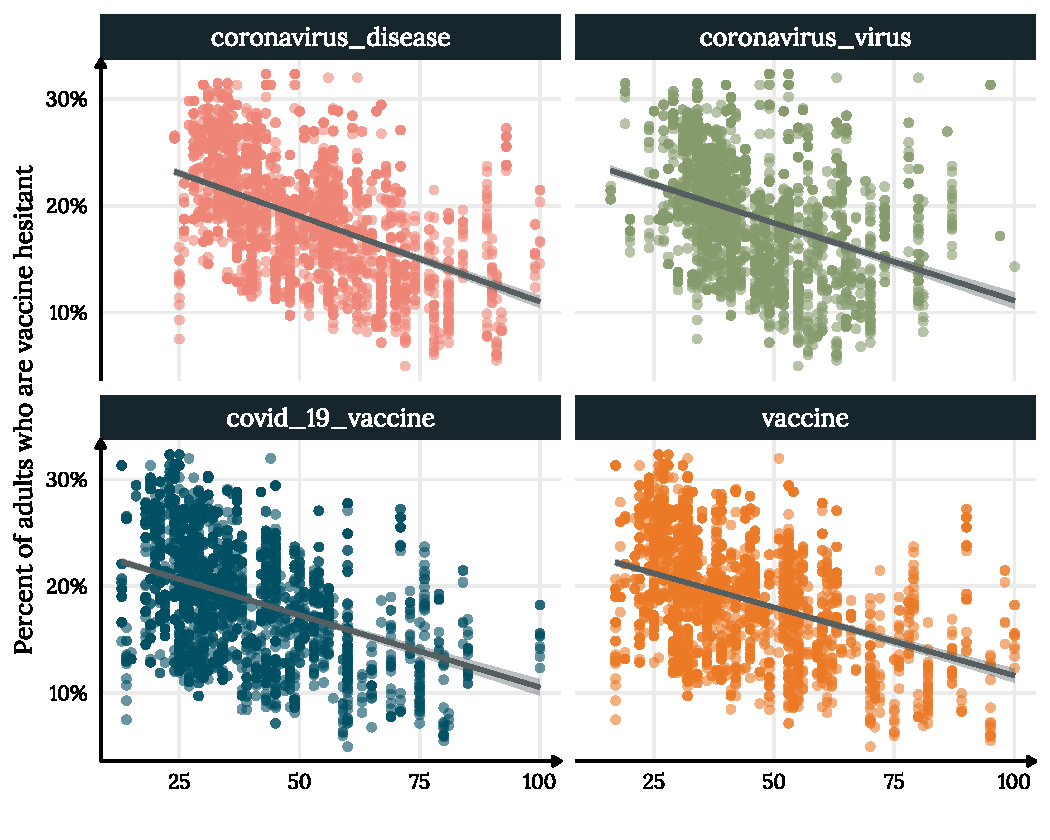
\includegraphics[width=0.8\linewidth]{figs/paper1/vacc_hes_plot-1.pdf}}
\caption{Vaccine hesitancy by each Google Trend with a fitted linear regression line}\label{fig:vacc_hes_plot}
\end{figure}


The second attitudinal measure I test is how Google Trends relates to rare mask
usage. As with vaccine hesitancy, the Pearson correlations are negligible.
Correlation's under |0.20| are negligible according to the
common standards. I introduce these trends in multiple linear regression in
table \ref{tab:mask_analysis}. Model 1 demonstrates that these five Google
Search Trends can explain about 8\% of the variance in mask usage across U.S.
counties, reinforcing the conclusion that the relationship is quite weak. The
coefficients themselves are significant in Model 1. However, after
including the demographic variables in Models 2 and 3, we see that the
relationship between the Google Search Trends and mask usage is strengthened in
magnitude and in significance, indicating a suppression effect due to
underlying relationships between the trends and demographic variables. While the
trends are significant and match the demographic variables in magnitude, the
low $r^2$ of 0.203 for the trends still provides evidence that Google Search
Trends data cannot replace survey analysis when trying to measure rare mask
usage.

\begin{table}[!h]

\caption{\label{tab:mask_analysis}Linear Regression Results for Rare Mask Usage}
\centering
\fontsize{8}{10}\selectfont

\begin{tabular}{lccc}
\toprule
  & Model 1 & Model 2 & Model 3\\
\midrule

Search for `Coronavirus Disease' & \num{-0.010}*** &  & \num{-0.012}***\\
 & (\num{0.003}) &  & \vphantom{1} (\num{0.003})\\
Search for `Coronavirus Virus' & \num{-0.012}*** &  & \num{-0.001}\\
 & (\num{0.003}) &  & (\num{0.003})\\
Search for `Cloth face mask' & \num{-0.009}* &  & \num{-0.015}***\\
 & (\num{0.004}) &  & (\num{0.004})\\
Search for `Mask' & \num{0.025}*** &  & \num{0.023}***\\
 & (\num{0.004}) &  & (\num{0.003})\\
Search for `Civil and political rights' & \num{-0.012}*** &  & \num{-0.008}***\\
 & (\num{0.002}) &  & (\num{0.002})\\
Total Population &  & \num{-0.012}*** & \num{-0.011}***\\
 &  & (\num{0.002}) & \vphantom{3} (\num{0.002})\\
Population Density &  & \num{-0.003}+ & \num{-0.004}*\\
 &  & (\num{0.002}) & \vphantom{2} (\num{0.002})\\
Unemployment Rate &  & \num{-0.028}*** & \num{-0.024}***\\
 &  & (\num{0.002}) & \vphantom{1} (\num{0.002})\\
\% over 65 &  & \num{-0.006}** & \num{-0.003}+\\
 &  & (\num{0.002}) & (\num{0.002})\\
\% below poverty line &  & \num{-0.010}** & \num{-0.009}**\\
 &  & (\num{0.003}) & \vphantom{2} (\num{0.003})\\
Median income &  & \num{-0.036}*** & \num{-0.030}***\\
 &  & (\num{0.003}) & \vphantom{1} (\num{0.003})\\
\% with broadband &  & \num{-0.006}* & \num{-0.007}**\\
 &  & (\num{0.003}) & (\num{0.003})\\
\midrule
Num.Obs. & \num{2964} & \num{3133} & \num{2954}\\
R2 & \num{0.077} & \num{0.176} & \num{0.203}\\
R2 Adj. & \num{0.076} & \num{0.174} & \num{0.200}\\
\bottomrule
\multicolumn{4}{l}{\rule{0pt}{1em}* p $<$ .05. ** p $<$ .01. *** p $<$ .001 (two-tailed test).}\\
\end{tabular}
\end{table}
\begin{figure}[h]
{\centering 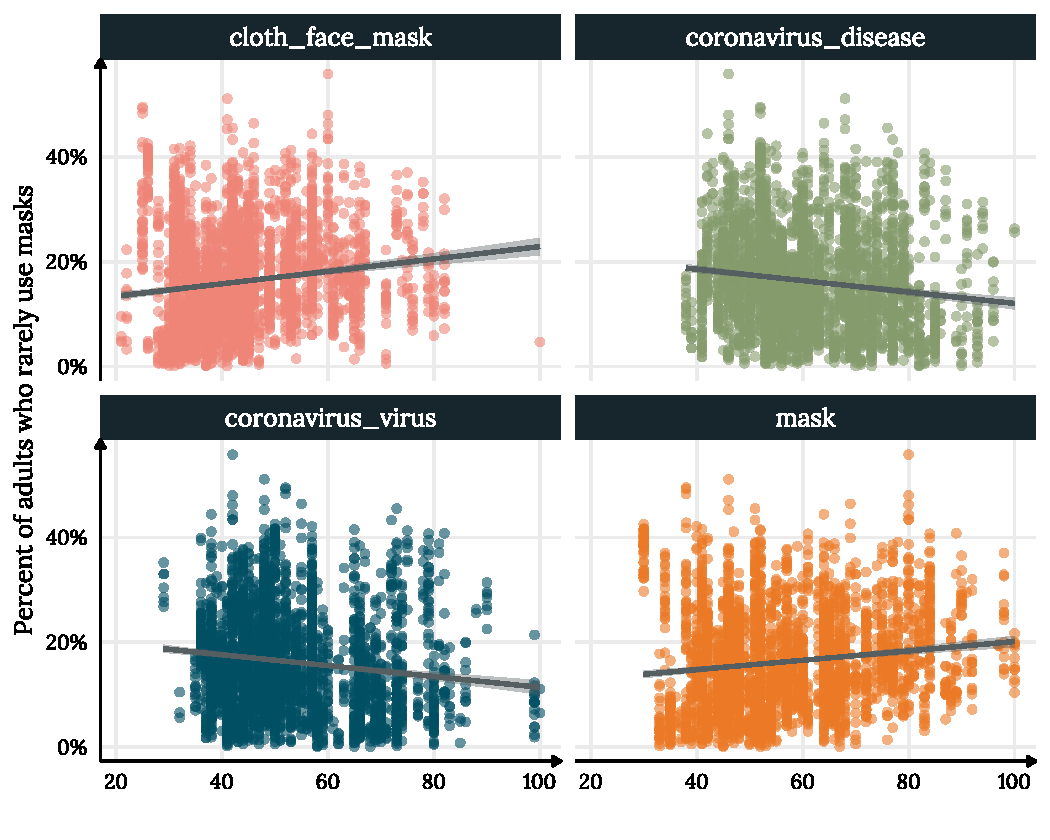
\includegraphics[width=0.8\linewidth]{figs/paper1/mask_plot-1.pdf}}
\caption{Rare mask usage by each Google Trend with a fitted linear regression line}\label{fig:mask_plot-1}
\end{figure}


\subsection{Validating Google Trends as metrics of health outcomes}

In addition to attitudinal measures, I attempt to validate Google Trends for
uses in the measurements of health indicators. The first indicator I assess is
COVID-19 case rates from 2020 through 2021. The Pearson correlation results
indicate negligible to weak relationships between the search terms and the
actual case rates across time and place. The repeated measures correlation
coefficient, a more reliable and less biased measure for longitudinal
correlations, reveals similarly weak results with a maximum correlation of 0.32
between 'smell loss' and rates of COVID-19. To further investigate the
relationship, I include the three trends in fixed effect hierarchical linear
models. Model 1 of Table \ref{tab:covid_analysis} indicates that the trends
themselves are able to explain about 20\% of the variation in COVID-19 rates
($r^2$ = 0.201). Few of the demographic variables influence COVID-19 rates in
models 2 or 3, though there is some suppression for median income, unemployment
rates, and population density. Model 3 has an $r^2$ of 0.200. I conclude that
the Google Trends are slightly related to COVID-19 rates, but that this
relationship is weak, and we should not attempt to use Google Trends as an
indicator of actual health outcomes.

\begin{table}[!h]

\caption{\label{tab:covid_analysis}Hierarchical Model for Covid Case Rates}
\centering
\fontsize{8}{10}\selectfont

\begin{tabular}{lccc}
\toprule
  & Model 1 & Model 2 & Model 3\\
\midrule
covid\_19 & \num{1.031}*** &  & \num{1.024}***\\
 & (\num{0.082}) &  & \vphantom{1} (\num{0.082})\\
smell\_loss & \num{7.373}*** &  & \num{7.374}***\\
 & (\num{0.082}) &  & (\num{0.082})\\
taste\_loss & \num{6.344}*** &  & \num{6.347}***\\
 & (\num{0.078}) &  & (\num{0.078})\\
covid\_rate\_fips\_mean & \num{0.813}*** & \num{0.982}*** & \num{0.879}***\\
 & (\num{0.019}) & (\num{0.010}) & (\num{0.020})\\
date & \num{0.029}*** & \num{0.038}*** & \num{0.029}***\\
 & (\num{0.000}) & (\num{0.000}) & (\num{0.000})\\
total\_pop &  & \num{0.064} & \num{0.409}**\\
 &  & (\num{0.066}) & (\num{0.140})\\
pop\_density &  & \num{0.010} & \num{0.463}***\\
 &  & (\num{0.067}) & (\num{0.123})\\
unemployment\_rate &  & \num{0.049} & \num{0.725}***\\
 &  & (\num{0.080}) & (\num{0.155})\\
over\_65 &  & \num{-0.116} & \num{-0.055}\\
 &  & (\num{0.074}) & (\num{0.139})\\
poverty\_rate &  & \num{0.054} & \num{0.351}\\
 &  & (\num{0.118}) & (\num{0.221})\\
median\_income &  & \num{0.031} & \num{0.907}***\\
 &  & (\num{0.114}) & (\num{0.214})\\
broadband &  & \num{0.073} & \num{0.437}*\\
 &  & (\num{0.097}) & (\num{0.182})\\
\midrule
Num.Obs. & \num{248346} & \num{284666} & \num{247655}\\
R2 Marg. & \num{0.201} & \num{0.081} & \num{0.200}\\
R2 Cond. &  & \num{0.081} & \\
\bottomrule
\multicolumn{4}{l}{\rule{0pt}{1em}Random intercept per county}\\
\multicolumn{4}{l}{\rule{0pt}{1em}* p $<$ .05. ** p $<$ .01. *** p $<$ .001 (two-tailed test).}\\
\end{tabular}
\end{table}
\begin{figure}[h]
{\centering 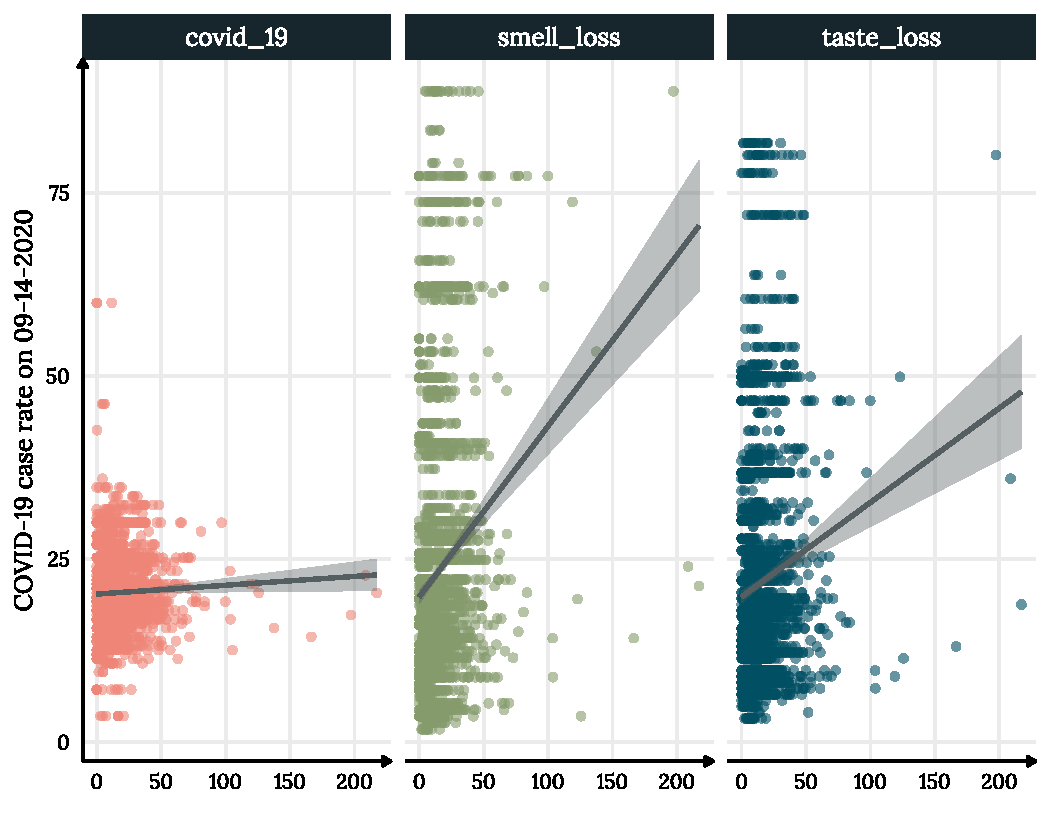
\includegraphics[width=0.8\linewidth]{figs/paper1/covid_plot-1.pdf}}
\caption{Covid case rate for 09-14-2020 by each Google Trend with a fitted linear regression line}\label{fig:covid_plot-1}
\end{figure}

Another health outcome I test is county suicide rates. As with previous cases,
there is only negligible correlation between actual suicide rates and Google
Search Trends, not exceeding 0.0845. In the more accurate repeated measures
correlation coefficient we see a maximum of 0.142 correlation, remaining
negligible. I introduce these trends into a fixed effect model to control for
inter-group variation over time in Table \ref{tab:suicide_analysis}. While table
\ref{tab:suicide_analysis} model 1 reveals a statistically significant
relationship between suicide hotline trends and suicide rates, the effect is
small, and the entire model only has an $r^2$ of 0.058. Adding in demographic
features in model 2 improves the $r^2$ to 0.56. In model 3, the inclusion of
Google Trends decreases the overall amount of suicide rate variance explained
compared to model 2. These analyses lead me to conclude that Google Search
Trends should not be used by researchers as indicators of suicide rates or
intentions.

% # TODO All variables have been standardized, right? So when you say an effect is ``small,'' could you give an illustration? E.g., translate it back into metric coefficients? For example, ''for every 100 additional calls to a suicide hotline, the suicide rate increases by x per 1,000 residents, according to the model,'' or something like that?  The main thing is to have an intuitive description of what the effect size is, not just to look at a standardized coefficient of .002.

\begin{table}[!h]

\caption{\label{tab:suicide_analysis}Fixed Effect Model for Suicide Rates}
\centering
\fontsize{8}{10}\selectfont

\begin{tabular}{lccc}
\toprule
  & Model 1 & Model 2 & Model 3\\
\midrule

Search for `Suicide' & \num{-0.001} &  & \num{-0.001}\\
 & (\num{0.001}) &  & \vphantom{2} (\num{0.001})\\
Search for `Depression' & \num{-0.001}+ &  & \num{-0.001}\\
 & (\num{0.001}) &  & \vphantom{1} (\num{0.001})\\
Search for `Suicide Hotline' & \num{0.002}*** &  & \num{0.002}***\\
 & (\num{0.001}) &  & (\num{0.001})\\
Year & \num{0.004}*** & \num{0.005}*** & \num{0.005}***\\
 & (\num{0.000}) & (\num{0.000}) & (\num{0.000})\\
Total Population &  & \num{-0.032}*** & \num{-0.027}**\\
 &  & (\num{0.010}) & (\num{0.009})\\
Population Density &  & \num{-0.037}** & \num{-0.033}**\\
 &  & (\num{0.011}) & (\num{0.011})\\
Unemployment Rate &  & \num{-0.001} & \num{-0.001}\\
 &  & (\num{0.001}) & \vphantom{1} (\num{0.001})\\
\% over 65 &  & \num{-0.010}*** & \num{-0.014}***\\
 &  & (\num{0.002}) & \vphantom{1} (\num{0.002})\\
\% below poverty line &  & \num{-0.005}*** & \num{-0.003}**\\
 &  & (\num{0.001}) & (\num{0.001})\\
Median income &  & \num{-0.014}*** & \num{-0.015}***\\
 &  & (\num{0.002}) & (\num{0.002})\\
\midrule
Num.Obs. & \num{30008} & \num{33582} & \num{30001}\\
R2 Marg. & \num{0.058} & \num{0.582} & \num{0.564}\\
\bottomrule
\multicolumn{4}{l}{\rule{0pt}{1em}Fixed intercept per county}\\
\multicolumn{4}{l}{\rule{0pt}{1em}* p $<$ .05. ** p $<$ .01. *** p $<$ .001 (two-tailed test).}\\
\end{tabular}
\end{table}
\begin{figure}[h]
{\centering 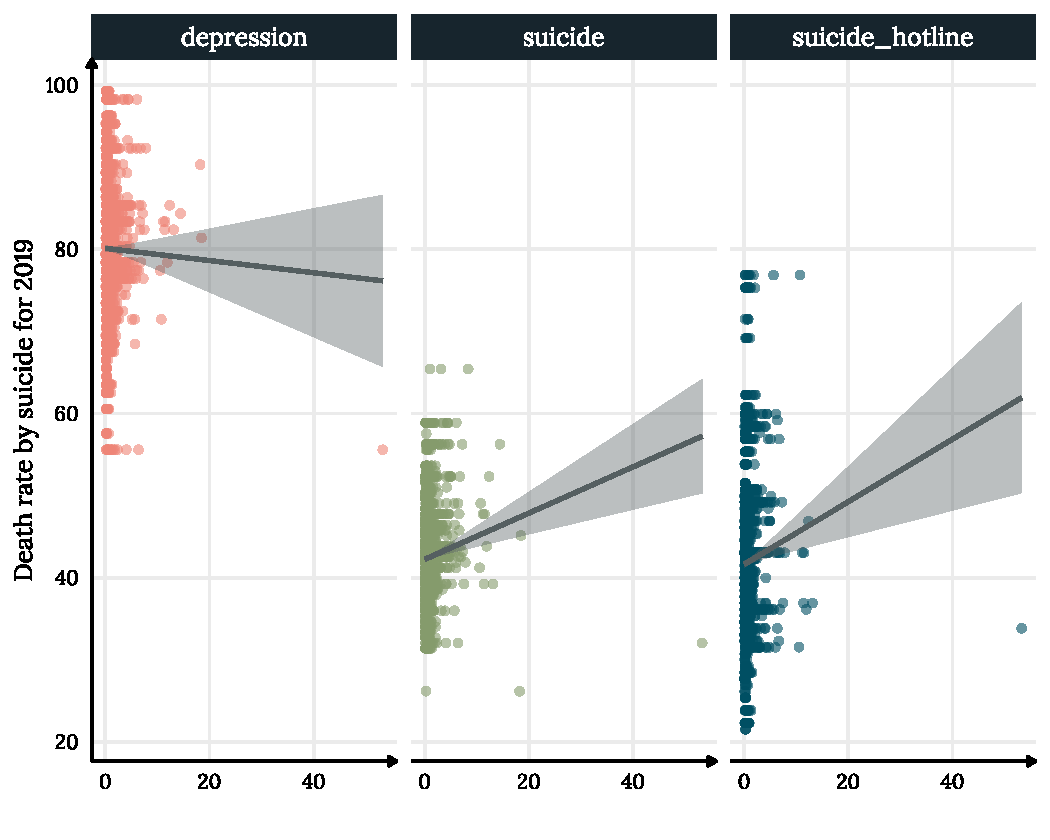
\includegraphics[width=0.8\linewidth]{figs/paper1/suicide_plot-1.pdf}}
\caption{Suicide death rate for 2019 by each Google Trend with a fitted linear regression line}\label{fig:suicide_plot-1}
\end{figure}

\subsection{Validating Google Trends as metrics of political support}

Previous research has shown some relationship between Google Search Trends and
political election results. I investigate the relationships between search trends
and U.S. Presidential Election results in 2016 and 2020. In 2016, Pearson
correlations of search trends with actual percentage of votes for Both Hilary
Clinton and Donald Trump do not exceed a |0.17| correlation for either candidate. In 2020,
results are even less related, with searches for neither Joe Biden nor Donald
Trump holding any real correlation with the 2020 results.

% The sign in Model 1 is interesting. The more likely a voter is to vote against Clinton, the more they search for her? (Obsessive?) Is that right? Also, I may be not seeing this correctly, but again I think I'd be interested in an interpretation in the original metrics of variables: ''According to Model 1, for every 1,000 searches for Clinton, she received X% less of the total actual vote,'' or something like that.
In Table \ref{tab:pres_2016_analysis}, I outline the results for the model
predicting the county percentage of votes for Hillary Clinton. Model 1
demonstrates how well Google Trends predict the votes; while the trend for
'Hillary Clinton' is significantly associated with votes, the model's $r^2$
($r^2$ = 0.027) shows that it does little to help explain the model variance. On
the other hand, adding in demographic features improves the model fit quite
well, bringing the $r^2$ up to 0.313 in model 2 and $r^2$ 0.327 in model 3.
Table \ref{tab:pres_2020_analysis} shows this same analysis for the 2020
election and predicts the percentage of votes for Joe Biden. While this model is
analogous to those in Table \ref{tab:pres_2016_analysis}, this model 1
demonstrates how unrelated Google Trends can be from actual outcomes. In
conclusion, I find that Google Trends are an unreliable and invalid indicator of
political support.

\begin{figure}[h]
{\centering 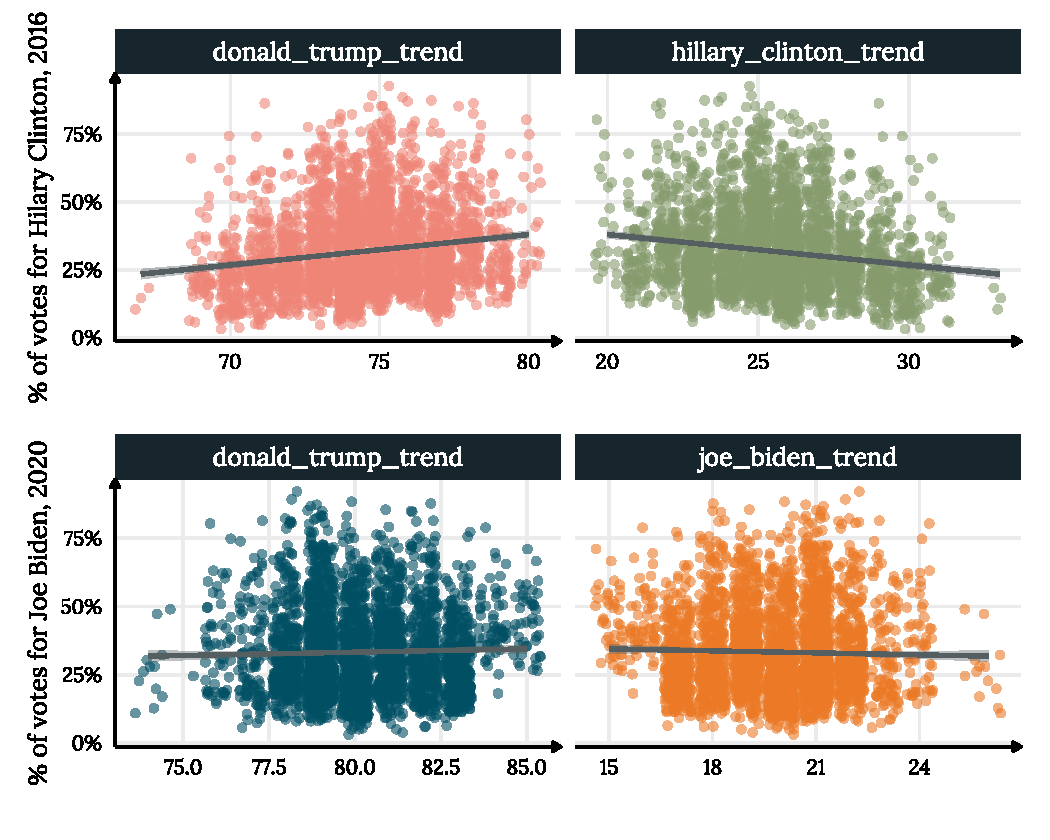
\includegraphics[width=0.8\linewidth]{figs/paper1/pres_plot-1.pdf}}
\caption{Presidential voting outcomes for 2016 and 2020 by each Google Trend with a fitted linear regression line}\label{fig:pres_plot-1}
\end{figure}

\begin{table}[!h]
\caption{\label{tab:pres_2016_analysis}}
\centering
\begin{tabular}[t]{}
\end{tabular}
\end{table}
\begin{table}[!h]

\caption{\label{tab:pres_2020_analysis}Linear Regression Results for 2020 Presidential Election Results (Joe Biden Shown)}
\centering
\fontsize{8}{10}\selectfont

\begin{tabular}{lccc}
\toprule
  & Model 1 & Model 2 & Model 3\\
\midrule

Search for `Joe Biden' & \num{-0.005} &  & \num{-0.014}***\\
 & (\num{0.003}) &  & (\num{0.002})\\
Total Population &  & \num{0.030}*** & \num{0.029}***\\
 &  & (\num{0.003}) & \vphantom{3} (\num{0.003})\\
Population Density &  & \num{0.021}*** & \num{0.022}***\\
 &  & (\num{0.003}) & \vphantom{2} (\num{0.003})\\
Unemployment Rate &  & \num{0.044}*** & \num{0.044}***\\
 &  & (\num{0.003}) & \vphantom{1} (\num{0.003})\\
\% over 65 &  & \num{-0.007}* & \num{-0.008}**\\
 &  & (\num{0.003}) & (\num{0.003})\\
\% below poverty line &  & \num{0.032}*** & \num{0.033}***\\
 &  & (\num{0.004}) & \vphantom{1} (\num{0.004})\\
Median income &  & \num{0.069}*** & \num{0.070}***\\
 &  & (\num{0.004}) & (\num{0.004})\\
\midrule
Num.Obs. & \num{3118} & \num{3118} & \num{3118}\\
R2 & \num{0.001} & \num{0.295} & \num{0.303}\\
R2 Adj. & \num{0.000} & \num{0.294} & \num{0.301}\\
\bottomrule
\multicolumn{4}{l}{\rule{0pt}{1em}Results predicting Donald J. Trump comparable and available upon request.}\\
\multicolumn{4}{l}{\rule{0pt}{1em}* p $<$ .05. ** p $<$ .01. *** p $<$ .001 (two-tailed test).}\\
\end{tabular}
\end{table}

\section{Discussion and Conclusion}
%TODO I’d say it is a test or assessment. Critique implies the answer is known a priori. I would focus on validation, note it it has implication (we need to test more and be more cautious),  and say future research should x,y,z. 

% The critique, is really about how and why we overlook being precisely incorrect if we like the aesthetics of an argument. I can think of some egregious examples.

% I would send the first paper to somewhere like soc methods or a stat journal, and the second to big data and society or the like.

% That said, there are things here that die hard stats people may find issues with. I also think a direct comparison of what google trends versus traditional survey data would predict would be very strong evidence of literally missing the mark.

% A related thought, is the assumption is the survey is right, since it is the referrant for validation. But often, the validation procedures of surveys can also lead to invalid claims. Cicourel wrote about this really well in 1982, and there are examples where a measure means totally different things to different respondents. E..g Alcohol may be read as ‘spiritis’ but not wine by some groups. So, it is possible that google is more accurate, and all these data sources require validation from interactions with humans in their lifeworld. That would be my position at least, but I think it is fair to say that the while the surveys have been more thoroughly tested, there are potential errors there as well.


This paper provides a test of the criterion validity of Google Trends for use in
Social Science. I failed to find correlation between the Google Trends and their
validated indicators. While some Google Trends tested were significantly
associated with the outcome in the linear regression model, effects tended to be
small and the total model interpretability remained low, even when
controlling for demographic variables.  

Some previous research has shown strong innovation in the computational social
sciences to gather sociodemographic data when survey or other research methods
are too costly \citep{blumenstockPredictingPovertyWealth2015}. Google Trends, in
theory, sounds like a promising data source to 'nowcast' attitudinal, health,
and political indicators. Not only would the data be easily and freely
accessible, but it would also provide indicators for areas where conducting
research may be too costly. The demand for this sort of indicator is clear and
fields like the health sciences have freely utilized this data source. However,
this article shows that Google Trends fails to map on to validated survey
metrics for attitudes, disease prevalence and political preferences. Social
scientists should not assume Google Trends data can serve as a replacement for
high quality survey data, at least for these measures.

As social scientists it is our responsibility to deeply investigate the validity
of the data that we use so we can be confident in our research findings. As with
any source of data, we must consider the potential pitfalls, especially in
research on using new methods and data sources
\citep{mcfarlandBigDataDanger2015}. In the case of Google Search Trends,
precaution is warranted.

%  TODO What might be some limitations of your analysis? Are there some issues raised here that should be further explored in subsequent research?